\section{原理}
X線回折による応力測定では,多結晶材料の結晶格子面間隔のひずみから応力を求める.本測定法は非破壊で計測でき,数十$\mathrm{\mu m}$オーダーの表面層の応力を計測できるなどの利点がある.

回折に与える結晶の格子面間隔を$d$,回折角$\theta$とするとBraggの式から
\begin{equation}
    2d\sin\theta = n\lambda
    \label{eq:braggの式}
\end{equation}
となる.式(\ref{eq:braggの式})を$\theta$で微分して格子面間隔$\Delta d$を求めると以下のようになる.
\begin{equation}
    \Delta d/d = -\cot\theta \cdot \Delta \theta
    \label{eq:delta_d}
\end{equation}
ここでひずみ$\epsilon_\phi$を,格子面間隔変位$\Delta d_\phi$,ひずみがない場合の格子面間隔$d_0$,回折角$\theta_0$とひずみが存在する場合の回折角$\theta_\phi$で近似的に表すと以下のようになる.
\begin{equation}
    \varepsilon_\phi = \Delta d_\phi /d_0 = -\cot\theta_0 \cdot (\theta_\phi - \theta_0)
    \label{eq:epsilon_phi}
\end{equation}
試料表面では表面層の応力を取り扱うので平面応力状態を仮定し,試料表面の測定位置を原点とすると,主ひずみ$\varepsilon_1$,$\varepsilon_2$,$\varepsilon_3$は,主応力$\sigma_1$,$\sigma_2$,$\sigma_3$,ポアソン比$\nu$,縦弾性係数$E$から次式で表される.
\begin{subequations}
    \begin{align}
        \varepsilon_1 &= (\sigma_1 - \nu\sigma_2)/E \label{eq:主ひずみ1} \\
        \varepsilon_2 &= (\sigma_2 - \nu\sigma_1)/E \label{eq:主ひずみ2} \\
        \varepsilon_3 &= -(\nu(\sigma_1 + \sigma_2))/E \label{eq:主ひずみ3}
    \end{align}
\end{subequations}
試料表面の直行座標系での応力$\sigma_x$,$\sigma_y$とひずみ$\varepsilon_x$,$\varepsilon_y$は,上式から
\begin{subequations}
    \begin{align}
        \varepsilon &= (\sigma_x - \nu\sigma_y)/E \label{eq:ひずみ_x} \\
        \varepsilon_y &= (\sigma_y - \nu\sigma_x)/E \label{eq:ひずみ_y} \\
        \varepsilon_z &= \varepsilon_3 = -\nu(\sigma_x + \sigma_y)/E \label{eq:ひずみ_z}
    \end{align}
\end{subequations}
となる.任意の$\Phi$,$\Psi$の方向に対するひずみ$\varepsilon_{\Phi\Psi}$は,$\varepsilon_1$,$\varepsilon_2$,$\varepsilon_3$により次式のように表される.
\begin{align}
    \varepsilon_{\Phi\Psi} &= \varepsilon_1\cos^2\Phi \sin^2\Psi + \varepsilon_2\sin^2\Phi\sin^2\Psi + \varepsilon_3\cos^2\Psi \notag \\
    &= (\varepsilon_1cos^2\Phi + \varepsilon_2\sin^2\Phi)\sin^2\Psi + \varepsilon_3(1 - sin^2\Psi) \label{eq:任意のひずみ}
\end{align}
ここで$\varepsilon_1cos^2\Phi + \varepsilon_2\sin^2\Phi$をより式(\ref{eq:任意のひずみ2})となり,右辺に式(\ref{eq:ひずみ_x})の$\varepsilon_3$と式(\ref{eq:ひずみ_z})の$\varepsilon_3$を代入して,式(\ref{eq:任意のひずみ3})となる.
\begin{equation}
    \varepsilon_{\Phi\Psi} = \varepsilon_xsin^2\Psi + \varepsilon_3(1 - sin^2\Psi)
    \label{eq:任意のひずみ2}
\end{equation}
\begin{equation}
    \varepsilon_{\Phi\Psi} = \{(1 + \nu)\sigma_xsin^2\Psi\}/E - \nu(\sigma_1 + \sigma_2)/E 
    \label{eq:任意のひずみ3}
\end{equation}
式(\ref{eq:任意のひずみ3})を$\sin^2\Psi$で微分し,$\varepsilon_\Psi = \varepsilon_{\Phi\Psi}$とすると,以下のようになる.
\begin{equation}
    \partial \varepsilon_\Psi/\partial \sin^2\Psi = \{(1 + \nu)\sigma_x\}/E
    \label{eq:ひずみの微分}
\end{equation}
したがって,式(\ref{eq:epsilon_phi})と式(\ref{eq:ひずみの微分})から,式(\ref{eq:応力_x})となる.
\begin{align}
    \sigma_x &= \{E/(1 + \nu)\} \cdot (\partial \varepsilon_\Psi/\partial \sin^2\Psi) \notag \\
    &= \frac{-Ecot\theta_0}{2(1 + \nu)} \cdot \frac{\pi}{180} \cdot \frac{\partial 2\theta_0}{\partial \sin^2\Psi} \notag \\
    &= KM
    \label{eq:応力_x}
\end{align}
式(\ref{eq:応力_x})より,$\sin^2\Psi$ー$2\theta$線図の勾配$M[\mathrm{deg}]$と,定数$K[\mathrm{MPa/deg}]$(応力定数)から応力$\sigma_x$を求めることができる.主な応力定数を表1に示す.
\clearpage
\begin{table}[htbp]
    \centering
    \caption{Stress constant method} % 表のキャプション
    \label{tbl:応力定数表} % 参照用ラベル
    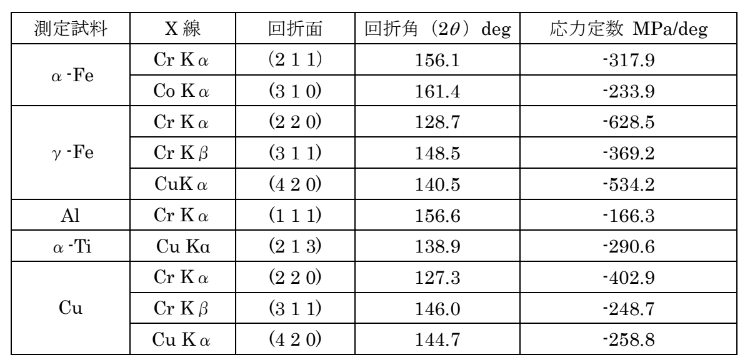
\includegraphics[width=0.8\textwidth]{fig/応力定数表.png} % 画像ファイル名と幅を指定
\end{table}
